\begin{savequote}[75mm]
In every discourse, whether of the mind conversing with its own thoughts, or of the individual in his intercourse with others, there is an assumed or expressed limit within which the subjects of its operation are confined. The most unfettered discourse is that in which the words we use are understood in the widest possible application, and for them the limits of discourse are co-extensive with those of the universe itself.
\qauthor{George Boole}
\end{savequote}

\chapter{Where we are}
\label{chap:where}

In this chapter we trace a smaller circle around our contributions, motivating our study, and reassessing its importance.

\section{Our vantage point}
% Now we can assess learning of timing in rats in the brain activity.
Electrode recording techniques have important limitations: They record only a small subset of neurons, and the specific neurons being recorded may change with passing days. While the low density of recordings can be bypassed with homogeneity assumptions, it makes harder to test hypothesis on recorded data, specially because the identity of neurons is transitional, and it is hard to guarantee we are measuring the same neurons for multiple days. One way to tackle the limitations is to compare recordings within shorter intervals, but this is only interesting if behavior changes fast, in the course of a single session. 

    \subsection{An unique task}
    % It was not possible. Problems. DRRD task
        Time learning is a slow process \cite{paton2018neural}. To study learning of temporal representations in the cortex, our group devised changes to the DRRD protocol that enabled learning to occur in a matter of one hour \cite{ReyesDRRD}. This new protocol enables us to compare the activity of the same neurons between moments in the session. 

    \subsection{Multivariate analysis techniques}
        To assess multidimensional representations, we should use multivariate techniques. Machine learning provides general multivariate techniques, capable of answering questions with little assumptions concerning the data. Instead of searching for a number of time cells or ramping neurons, we can ask about representation in a more general sense, and examine its presence in the recorded neural activity \cite{bakhurin2017differential}. 

% \section{Potential contributions}
% As introduced before, we will split our theoretical contributions into their corresponding level of analysis whenever possible. 
%     \subsection{Computational}
%     % Computational
%         % Taxonomy of timing
%         Multiple learning mechanisms seem to play their roles in animal behavior. 
%     \subsection{Algorithmic}
%     % Algorithmic
%         % processes
%         % learning mechanisms
%     \subsection{Implementational}
%     % Implementational
%         % brain regions
%         % neural correlates

\section{Objectives}
    % Preparar o leitor:
    %   Um dos objetivos é fazer uma discussão sobre a perspectiva 
    %   atual dos modelos, teoria e etc. Revisão do arcabouço teórico, estado da arte, etc. Construção de pontes. 
    % Timing mechanisms?
    The current work has two main objectives. On the one hand, we want to understand how time representations develop with training, to assuage the lack of experimental evidence regarding this fundamental question. On the other hand, we want to further locate the timing literature in the broader scope of the learning literature.
    
    In detail, we have the following objectives:
    \begin{enumerate}
        \item To compare the presence of time representations before and after learning in the medial Pre Frontal Cortex (mPFC) and in the Striatum.
        \item To make sense of experimental results using the theoretical framework of timing and using the theoretical framework of learning.
    \end{enumerate}


\section{Hypothesis}
    We expected the quality of time-representation to increase with training, and did not expected any specific distinctions between mPFC and Striatum, even though we wanted to explore the possibility. This was motivated by studies that revealed the presence of time representations in proficient animals \cite{bakhurin2017differential,buhusi2018inactivation}.
    
    \begin{figure}
        \centering
        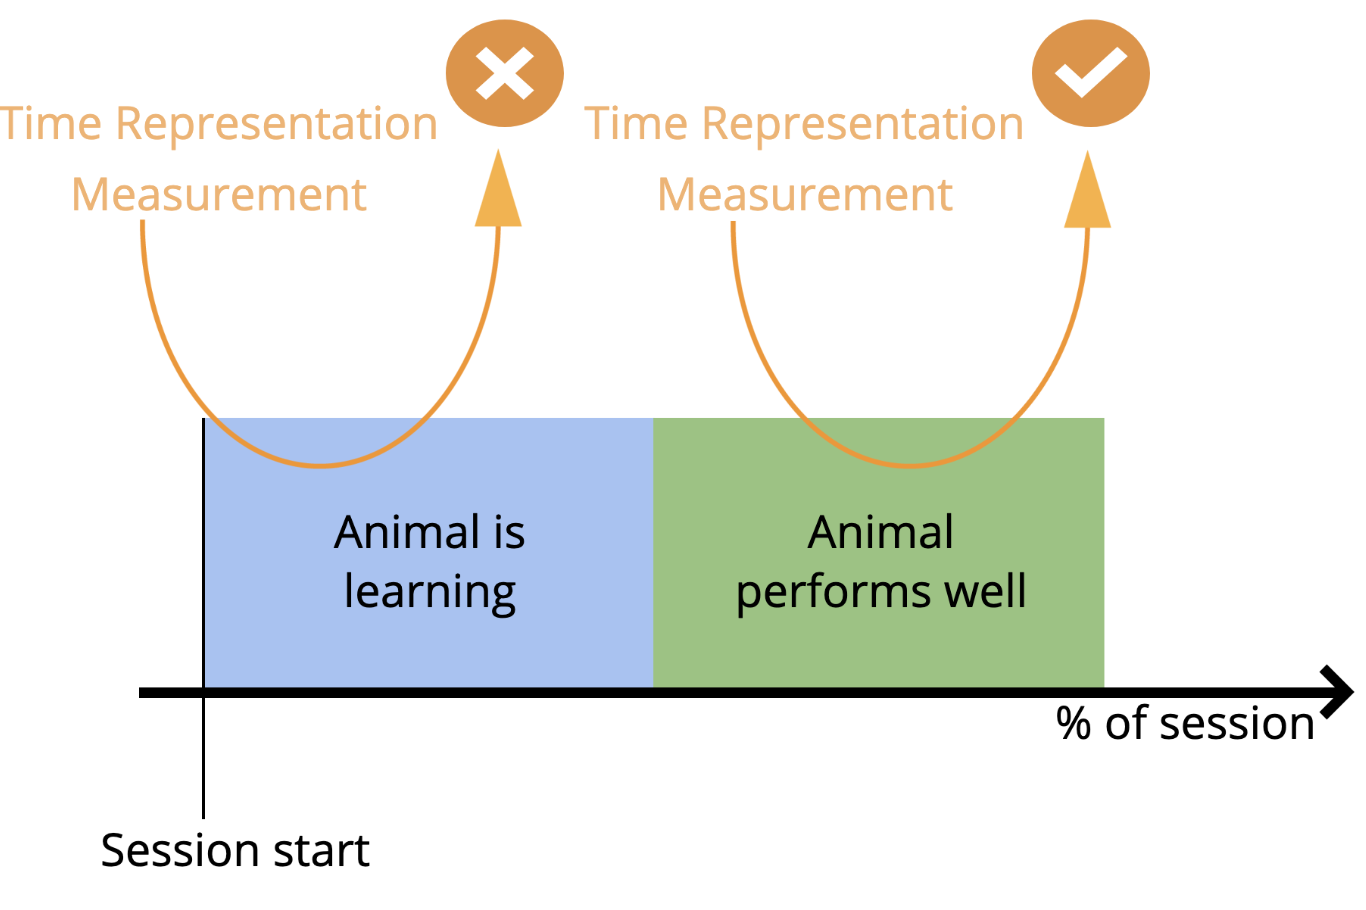
\includegraphics[width=0.8\textwidth]{figures/sketches/hypothesis.png}
        \caption[Visual sketch of our hypothesis.]{Schematics of our hypothesis. We expected that, during learning, the representation would be weak or absent, and stronger when the animal started performing well.}
        \label{fig:hip}
    \end{figure}
    
    
    Concerning the relative location of timing and learning, we expected to establish a comparative measure between the functioning of the mPFC and STR.
    
